\message{ !name(Mansfield-CS375-WK5.tex)}\documentclass[12pt]{article}
\usepackage[latin1]{inputenc}
\usepackage{amsmath}
\usepackage{mathtools}
\usepackage{xspace}
\usepackage{graphicx}
\usepackage[english]{babel}
\usepackage[font=small,labelfont=bf]{caption}
\usepackage[centering,includeheadfoot,margin=2cm]{geometry}
\usepackage{tikz}
\usetikzlibrary{shapes,arrows,automata,trees}
\title{CS375 WK5}
\author{Jason N Mansfield}
\begin{document}

\message{ !name(Mansfield-CS375-WK5.tex) !offset(-3) }




\begin{figure}
\begin{center}
\caption{Q01: $L_1$ = (a+b)*a}
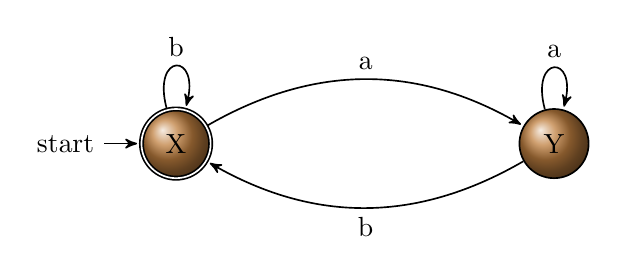
\begin{tikzpicture}[->,>=stealth',shorten >=1pt,auto,node distance=4.8cm, semithick]
\tikzstyle{every state}=[draw=black,text=black, ball color=brown]
\node[initial,state,accepting] (X) {X};
\node[state][right of=X](Y){Y};
\path (Y)edge [bend left] node{b}(X)
         edge  [loop above]node{a}(Y)
      (X)edge [loop above]node{b}(X)
         edge [bend left] node{a}(Y);
\end{tikzpicture} 
\end{center}
\end{figure}

\begin{figure}
\begin{center}
\caption{Q01: $L_2$= b(a+b)*}
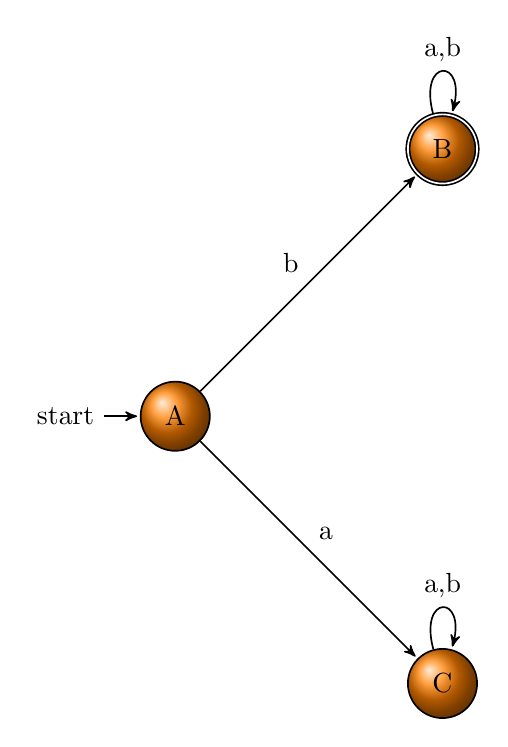
\begin{tikzpicture}[->,>=stealth',shorten >=1pt,auto,node distance=4.8cm, semithick]
\tikzstyle{every state}=[draw=black,text=black, ball color=orange]
\node[initial,state] (A) {A};
\node[state,accepting][above right of=A](B){B};
\node[state][below right of=A](C){C};
\path (A)edge node{b}(B)
         edge  node{a}(C)
      (B)edge  [loop above]node{a,b}(B)
      (C)edge [loop above]node{a,b}(C);
\end{tikzpicture} 
\end{center}
\end{figure}



\end{document}
\message{ !name(Mansfield-CS375-WK5.tex) !offset(-55) }
